% !TeX encoding = UTF-8
% !TEX root = ../presentation.tex
\section{Referencial Teórico}
   \subsection{{\it Field-Programmable Logic Device} (FPGA)}
      %\frame{\centering \bf \Huge \color{beamerCinza} \textit{Field-Programmable Logic Device}}
      % uso de fpga no mundo
      \begin{frame}{FPGA} \vspace{-1em}
         \begin{itemize}
            \setlength{\itemsep}{1.2em}
            \item FPGAs eram utilizados unicamente na protitipação ASIC.
            
            \item Mas com a elevação do custo de engenharia não recorrente\footnote{NRE, que refere-se ao custo de pesquisa, \design, desenvolvimento e teste de um novo produto e exigências de mercado.}.
            
            \item Interessou-se na utilização de FPGAs para SE devido \cite{Mei2000}:
            \begin{itemize}
               \item Suas vantagens em termos de flexibilidade de projeto e;
               \item Custo zero de engenharia não recorrente citada
            \end{itemize}
         
            \item Entretanto, enquanto configurar um \hardware\ reconfigurável é uma tarefa fácil graças às ferramentas disponíveis hoje, \emph{criar um \design\ de \hardware\ inicial não é} \cite{Sass2010}.
            
         \end{itemize}
      \end{frame}
   
   \begin{frame}
      \begin{figure}[h] \centering
         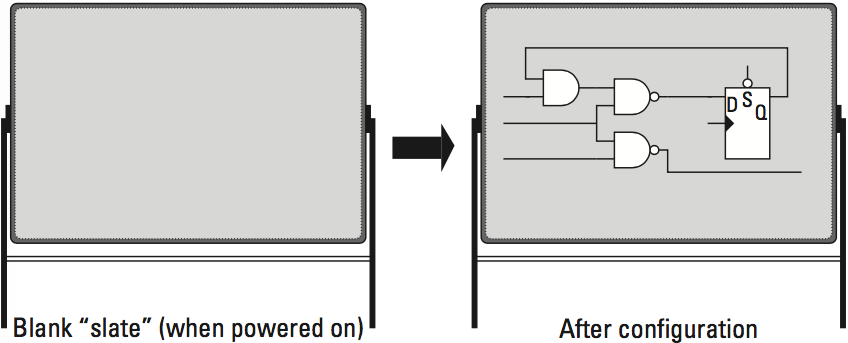
\includegraphics[width=1\textwidth]{img/rt-board.png}
         \caption{Ilustração em alto nível do funcionamento interno do FPGA. Fonte: \cite{Sass2010}.}
      \end{figure}
      \pdfnote{Permite ao \designer\ de SE ter uma \textit{lousa branca} em que possa  implementar}
      \pdfnote{\hardwares\ computacionais personaliz tão facilmente como o desenvolvim de um \software}
   \end{frame}

   \begin{frame}{Tecnologia dos FPGA} \vspace{-1em}
      \textbf{Vários módulos lógicos programáveis} relativamente \textbf{pequenos} e independentes, interconectados.
      
      \begin{itemize}
         \item A maioria dos FPGAs utilizam \textit{look-up table} (LUT) para criar as funções lógicas desejadas.
         \begin{itemize} 
            \setlength{\itemsep}{1.5em}
            \item Uma LUT funciona como uma tabela-verdade, ou seja, registradores programáveis. 
            \item Cada módulo lida com até quatro ou cinco variáveis de entrada;
            \item A saída é programada para criar a função combinacional armazenando valores verdadeiros e falsos adequado a cada combinação de entrada;
            \item Eles não são associados a nenhum pino de entrada e saída (I/O, do inglês \textit{Input and Output}). 
         \end{itemize}
      
      \end{itemize}
      \pdfnote{pequenos pra criar funções +}
   \end{frame}
   
   
   \begin{frame}{Tecnologia dos FPGA} \vspace{-1em}
      Vários módulos lógicos programáveis relativamente \textbf{pequenos} e \textbf{independentes}, \textbf{interconectados}.
      
      \begin{itemize}
         \setlength{\itemsep}{1.2em}
         
         \item Os recursos de roteamento de sinal programável dentro do chip
         \begin{itemize}
            \item Os atrasos de sinal em um projeto dependem do roteamento real de sinal selecionado pelo \software\ de programação. 
         \end{itemize}
         
         \item Pinos de I/O são conectados ao bloco programável de entrada e saída que, por sua vez, é conectado aos módulos lógicos com linhas de roteamento selecionadas.
            \bigskip
         \item Assim, FPGAs são chips que podem ser programados instantaneamente para funções de qualquer circuito digital \cite{Choi2016}.   
      \end{itemize}
      \pdfnote{pequenos pra criar funções +}
   \end{frame}

   \begin{frame}{Tecnologia dos FPGA} \vspace{-1em}
      \begin{columns}
         \begin{column}{0.6\textwidth}
            \begin{figure}[h] \centering
               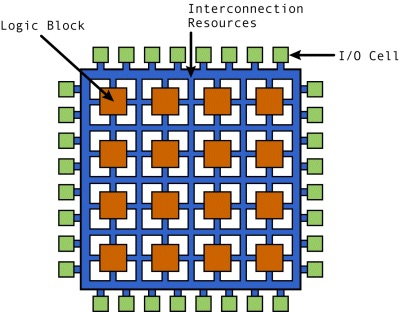
\includegraphics[width=1\textwidth]{img/rt-arch_fpga.jpg}
               \caption{Exemplo da arquitetura internas de um FPGA. Fonte: \url{http://www.eetimes.com/document.asp?doc_id=1274496}. Acesso: 30/05/2017.}
            \end{figure}
         \end{column}
         \begin{column}{0.4\textwidth}
            Hoje, esses dispositivos possuem \cite{Choi2016}
            \begin{itemize}
               \setlength{\itemsep}{1.2em}
               \item Mi de portas de lógica programável;
               \item Bi transistores;
               \item Blocos de \hardware\ dedicados dedicados como
               \begin{itemize}
                  \setlength{\itemsep}{0.8em}
                  \item Memórias embarcadas;
                  \item Multiplicadores de ponto-fixo.
               \end{itemize}
            \end{itemize}
         \end{column}
      \end{columns}
      \pdfnote{Tornando-o um dos (CI) MAIS densos existente.}
   \end{frame}

   \begin{frame}{Tecnologia dos FPGA} \vspace{-1em}
      Segundo \cite{tocci2003sistemas}
      \begin{itemize}
         \setlength{\itemsep}{1.5em}
         \item Podem fornecer uma série de opções de projeto sendo voltados para indústria e até mesmo educação.
          
         \item Ao utilizar tecnologia CMOS, o consumo de energia é relativamente baixo comparado com outras tecnologias
         \begin{itemize}
            \item Pode-se confeccionar em nível de tensão elétrica, frequências e cargas para os sinais de I/O. 
         \end{itemize}
      
         \item O mercado fornece diferentes graus de velocidade de FPGA a fim de que o projetista utilize o mais adequado ao projeto. 
         
         \item Entretanto, um dispositivo FPGA pode ser configurado para um número infinito de projetos.
         \begin{itemize}
            \item Não é possível afirmar o montante de dissipação de energia para um dispositivo FPGA.
         \end{itemize}
         
      \end{itemize}
      \pdfnote{tecnologia e energia}
      \pdfnote{Quartus estima ouso de energia. }
   \end{frame}

   \begin{frame}{Tecnologia dos FPGA} \vspace{-1em}
      
      \begin{itemize}
         \setlength{\itemsep}{1.2em}
      % Importancia
         \item Ao utilizar FPGA, é possível obter inúmeras vantagens \cite{tocci2003sistemas, Plessl2003}
         \begin{itemize}
            \setlength{\itemsep}{1.5em}
            \item Como são dispositivos programáveis, a mesma funcionalidade pode ser obtida com um CI ao invés de diversos circuitos individuais;
               \bigskip
            \item Maior confiabilidade;
            \item Menor espaço ocupado na placa, consumo de energia, complexidade de desenvolvimento e, geralmente, menor custo de fabricação.
         \end{itemize}
      \end{itemize}
   \end{frame}

   \begin{frame}{\textit{Hard} e \textit{Software Cores}} \vspace{-1em}
      A CPU pode ser implementada em duas formas, sendo estas \textit{hard} e \textit{soft} \cores\ \cite{Plessl2003}. 
      \begin{itemize}
         \setlength{\itemsep}{0.5em}
         \item \textbf{\textit{Hard Core}:} \core\ dedicado;
         \item \textbf{\textit{Soft Core}:} feito por meio da sintetização e mapeamento de um processador no FPGA com seus recursos lógicos. 
      \end{itemize}
   
      \begin{figure}[h] \centering
         \vspace{-8pt}
         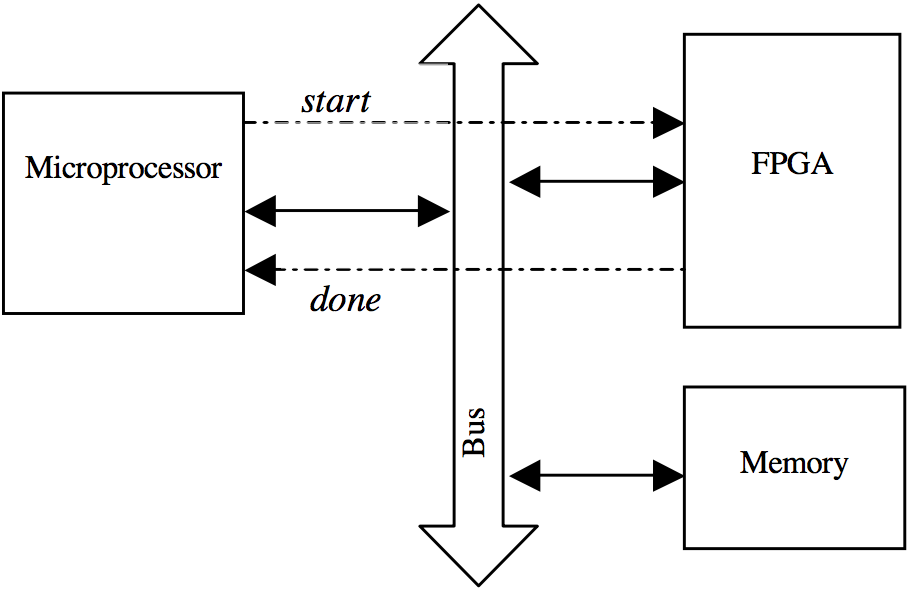
\includegraphics[width=0.65\textwidth]{img/into-soc.png}
         \caption{Visão geral de um SoC FPGA.}
         \label{fig:rb-soc}
      \end{figure}
   
      \pdfnote{HC: um pedaço de CI dentro (ou não) de um FPGA}
      \pdfnote{SC: é obtido por meio de \design\ e sintetização na placa }
      \pdfnote{vantags:}
      \pdfnote{usar todos recursos, máxima performance}
      \pdfnote{permite a extensão da arquitetura}
      \pdfnote{-> HDL}
   \end{frame}

   \begin{frame}{\textit{Hardware Description Language} (HDL)} \vspace{-1em}
      \begin{itemize}
         \setlength{\itemsep}{0.8em}
         \item Classes de linguagens de computação usados para descrever formalmente um circuito eletrônico.
         
         \item É capaz de descrever o comportamento temporal ou a estrutura de circuito (espacial) de um sistema eletrônico. 
         \begin{itemize}
            \item Origem: documentação do comportamento do \hardware\ \cite{Sass2010}.
         \end{itemize}
         
         \item Amplamente utilizada em \design\ de \hardware
         
         \begin{itemize}
            \item Pois possui detalhação altíssima do \hardware.
         \end{itemize} 
      
         \item A utilização de uma HDL é o primeiro passo no processo de síntese em FPGA \cite{Smith1998}. 
         \begin{itemize}
            \item A propriedade única deste é que, com esse processo de síntese, é possível alterar o código HDL, e sintetizar no mesmo dispositivo para testar;
            \item Quantas vezes forem necessárias, sem custo adicional.
         \end{itemize}
         
        \item Maioria de engenheiros utilizam-na.
        \begin{itemize}
           \item Mas possuem um nível elevado de complexidade \cite{Choi2016}, existe outras linguagens disponíveis para uso \cite{Sass2010}. 
        \end{itemize}
      \end{itemize}
   \end{frame}


   \begin{frame}{\textit{Hardware Description Language} (HDL)} \vspace{-1em}
      \begin{itemize}
         \setlength{\itemsep}{1.7em}
         \item Sintetizador em Alto Nível (HLS) são procedimentos que sintetizam códigos em alto nível para HDLs \cite{Choi2016}.
         \begin{itemize}
            \setlength{\itemsep}{1.2em}
            \item Podem reduzir os longos ciclos do processo de \design\ de \hardware\ e ainda;
            \item Trazer melhoria em performance e eficiência energética.
         \end{itemize}
         
         \item Ferramentas como o \textit{framework} LegUp e OpenCL \cite{Trevett2008}.
         \begin{itemize}
            \setlength{\itemsep}{1.2em}
            \item Entregar um bom HLS;
            \item Amenizar esses problemas de projetos
         \end{itemize} 
      \end{itemize}
   \end{frame}


   \begin{frame}{HLS} \vspace{-1em}
      LegUp High-Level Synthesis.
      \begin{itemize}
         \setlength{\itemsep}{0.7em}
         \item Programa padrão \textit{C} como entrada e automaticamente compila o programa para dispositivos FPGA \cite{Canis2011}.
         \begin{itemize}
            \item Totalmente em \hardware\ e outros híbridos (\textit{hard} e \textit{soft cores}).
         \end{itemize}
      \end{itemize}
   
         \bigskip
         
      OpenCL.
      \begin{itemize}
         \setlength{\itemsep}{1.2em}
         \item API comum para execução de programas em sistemas heterogêneos.
         \begin{itemize}
            \item Processadores \textit{multicores}, GPUs ou outros aceleradores \cite{Shagrithaya2013, Czajkowski2012}. 
         \end{itemize}
         
         \item Nível de paralelismo em tarefas e dados. 
         
         \item Define-se um \core\ \textit{Runtime Environment} e seus dispositivos.
         
      \end{itemize}
      \pdfnote{bib \textit{multi-threads} \textit{Pthread}, \textit{OpenMP} aceler. }
   \end{frame}

   
   \subsection{{\it Profile}}
   %\frame{\centering \bf \Huge \color{beamerCinza} \textit{Profile}}

   \begin{frame}{\textit{Profile}} \vspace{-1em}
      %\begin{itemize}
       %  \item 
      %\end{itemize}
      
      \begin{columns}
         \begin{column}{0.5\textwidth}
            
            \begin{figure}[h] \centering
               \vspace{-24pt}
               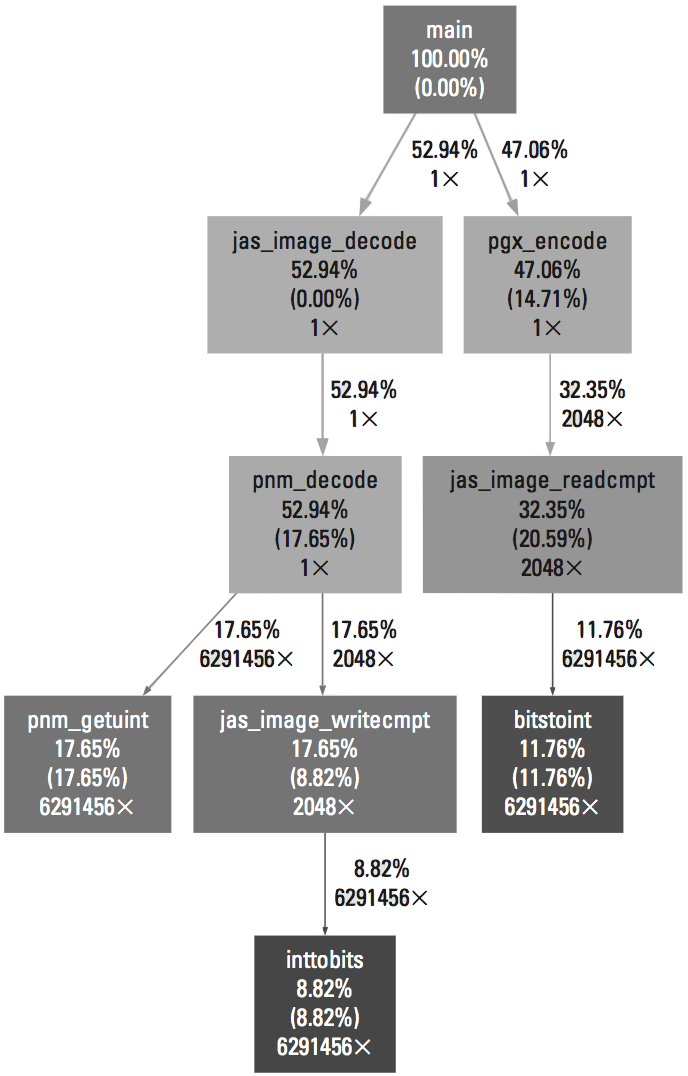
\includegraphics[width=0.8\textwidth]{img/f4-1-2.png}
               \caption{\Profile\ da codificação de imagem em formato JPEG. Fonte: \cite{Sass2010}.}
            \end{figure}
         \end{column}
         \begin{column}{0.5\textwidth}
            \vspace{-1cm}
            \begin{itemize}
               \setlength{\itemsep}{1.5em}
               \item Realiza-se interrupções periódica no programa e amostra o seu \textit{program counter}
               \begin{itemize}
                  \setlength{\itemsep}{1em}
                  \item Utiliza-se de um histograma para contar o endereço particular;
                  
                  \item E assim, calcular a fração aproximada do tempo total de execução gasto em suas partes. 
               \end{itemize}
               
               \item Distribuições GNU/Linux possuem a ferramenta \texttt{gprof} na qual realiza o cálculo de tais informações de \software\ \cite{Graham1982}.
            \end{itemize}
         \end{column}
      \end{columns}
      \pdfnote{coletar info em tempo de execução.}
      \pdfnote{soft entrada, mensura-se seu tempo.}
      
   \end{frame}


   \subsection{Sistemas Computacionais \Wearables}
      %\frame{\centering \bf \Huge \color{beamerCinza} \textit{Sistemas Computacionais \Wearables}}

      \begin{frame} {Sistemas Computacionais \Wearables} \vspace{-1em}
         % Introdução histórica e geral
         \begin{block}{Definição \cite{Amorim2017}:} 
            Com a possibilidade de ter um computador acoplado ao corpo, proporciona-se ao usuário um nível de informações contextualizadas dentro de um ambiente interativo.
         \end{block}
            
            \bigskip
      
         \begin{block}{Definição \cite{Gemperle1998}:} 
            Quando possui sua `\textit{wearability}' sendo este definido como a interação entre o corpo humano e o objeto \textit{wearable} estendendo ao corpo em movimento.
         \end{block}
      
         
      \end{frame}
   
   
   \begin{frame} {Sistemas Computacionais \Wearables} \vspace{-1em}
      \begin{itemize}
         \setlength{\itemsep}{1.5em}
         \item Introduzido em 1968 e novamente em 1996 e 1997 \cite{Sutherland1968, Mann1996, Mann1997}
         
         \item Entretanto, foi depende diretamente da miniaturização dos módulos eletrônicos. 
         
         \item Exemplo: \textit{smartwatches}, \textit{fitness trackers}, óculos, equipamentos de VR e AR, nas indústrias e nas atividades pessoais de usuários. 
         
         \item Dados de teclados ou \textit{display} LCD contradiz com o paradigma de operações \textit{hands-free} e a propriedade de computação \wearable\ discreta \cite{Plessl2003}.
         \begin{itemize}
            \setlength{\itemsep}{0.5em}
            \item Tais componentes são \textit{prestadores de auxílio à tarefas pessoais de usuários}.
            \item Sistemas distribuídos construídos a partir desses equipamentos interativos são \textit{ineficientes}.
            \begin{itemize}
               \item Falta-se a especialização de \textit{componentes individuais de propósito específico}.
            \end{itemize}
         \end{itemize}
      \end{itemize}
   \end{frame}

   \begin{frame}{Sistemas Computacionais \Wearables}
      \begin{itemize}
         \item Sendo miniaturizados, aumenta-se a sua atração devido à
         
         \begin{itemize}
            \setlength{\itemsep}{2.0em}
            \item Fácil disponibilidade dos dispositivos;
            \item Preço baixo;
            \item Ferramentas de desenvolvimento aplicações específicas incluindo compiladores e sistemas operacionais, mas não são otimizados para uso \wearable.
         \end{itemize}
         
      \end{itemize}
   \end{frame}
   
      \begin{frame}{Sistemas Computacionais \Wearables} \vspace{-1em}
         \begin{columns}
            \begin{column}{0.6\textwidth}
               \begin{figure}[h] \centering
                  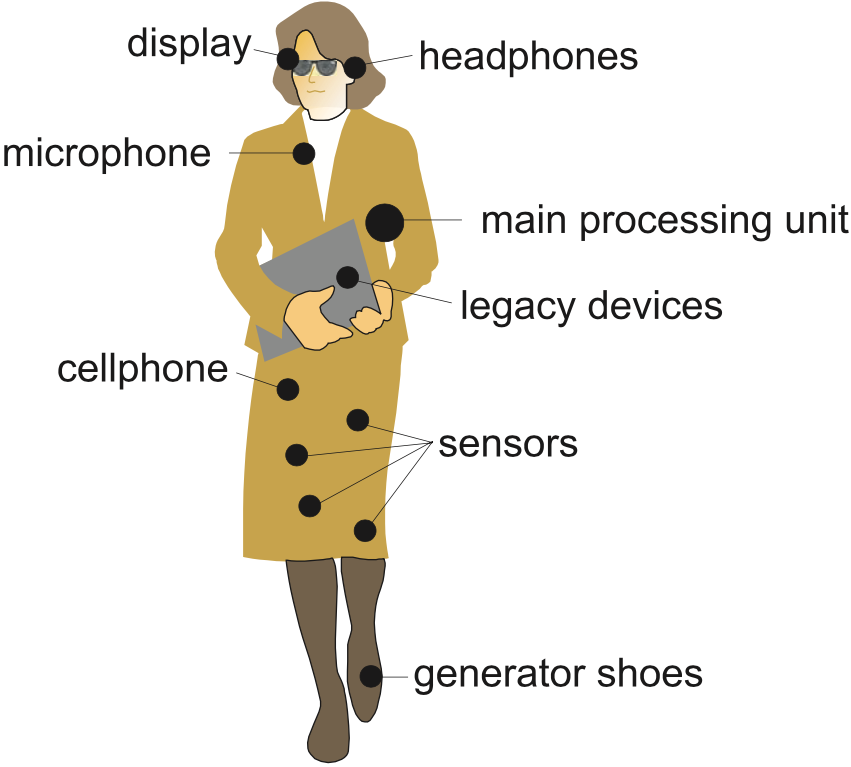
\includegraphics[width=1\textwidth]{img/into-wearable2.png}
                  \caption{Exemplificação de alguns dispositivos \wearables. Fonte: \cite{Plessl2003}.}
                  \label{fig:into-wearable}
               \end{figure}
            \end{column}
            \begin{column}{0.4\textwidth}
               Distribuição espacial dos módulos pelo corpo, a comunicação:
               \begin{itemize}
                  \setlength{\itemsep}{1.5em}
                  \item Torna-se importante no consumo de energia \cite{Kymissis1998}.
                  \item Pode ser mista, entre conexões cabeadas e sem-fios, mas a predominância sem-fio por causa da mobilidade \cite{Plessl2003}.
               \end{itemize}
               
            \end{column}
         \end{columns}
         
      \end{frame}
   
   
      % Característica de um dispositivo wearable
      \begin{frame}{Características de um \Wearable}
         \begin{itemize}
            \item Caracteriza-se um \wearable\ acordando às classificações pré-estabelecidas em relação à suas funcionalidades e requisitos de \hardware. 
            \begin{itemize}
               \setlength{\itemsep}{1.5em}
               \item Mesmo existindo inúmeros modelos e características diferentes, muitas soluções em \hardware\ compartilham uma arq. e org. interna de recursos comum.
               
               \item Também podem ser expandidos às características de OS \cite{Delabrida2016, Amorim2017}.
               
            \end{itemize}
         \end{itemize}
 
         \begin{figure}[h] \centering
            \vspace{-5pt}
            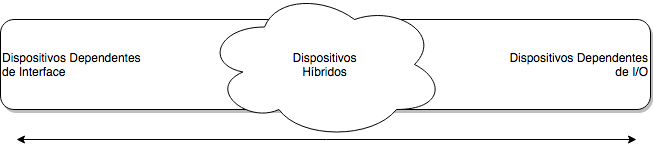
\includegraphics[width=0.9\textwidth]{img/rt-gradiente.png}
            %\vspace{-10pt}
            \caption{Classificação de \wearables. Fonte: Adaptado de \cite{Amorim2017}.}
         \end{figure}
      \end{frame}
   
   \begin{frame}{Características de um \Wearable} \vspace{-1em}
      
      \begin{figure}[h] \centering
         \vspace{-5pt}
         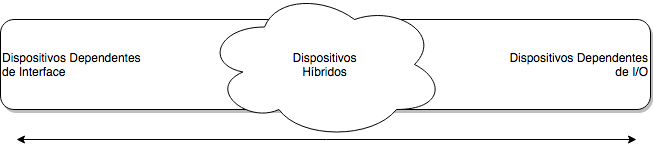
\includegraphics[width=0.9\textwidth]{img/rt-gradiente.png}
         %\vspace{-10pt}
         \caption{Classificação de \wearables. Fonte: Adaptado de \cite{Amorim2017}.}
      \end{figure}
      \begin{itemize}
         \setlength{\itemsep}{1em}
         \item A separação dos conceitos computação \wearable\ e IoT ainda não estão claros segundo a bibliografia. 
         
         \item OS para \wearable\ são comumente focado em um único tipo de seguimento de produto como os \textit{smartwatches}, proporcionando aos desenvolvedores um meio para sua aplicação final além de um produto de alta qualidade.
         
         \item Também, atualmente, não existe nenhum sistema que satisfaça todos os requisitos de todas as classificações \cite{Amorim2017}.
      \end{itemize}
   \end{frame}

   \begin{frame}{Características de um \Wearable} \vspace{-1em}
      \begin{itemize}
         \setlength{\itemsep}{1.5em}
         \item Já \cite{Jozwiak2017} caracteriza como um sistema \textit{cyber}-físico\footnote{Sendo \textit{cyber-} uma combinação dos termos `computador', `rede de computadores' ou `realidade virtual' com um segundo termo, no caso o `físico' oriundo de circuitos.} móvel autônomo.
         
         \item Podem ser utilizados para aplicações de consumidores, extensões ou reposição de capacidades humanas, ou industriais
         
         \item Representam uma grande parte da heterogeneidade de sistemas embarcados, 
         \begin{itemize}
            \setlength{\itemsep}{1.0em}
            \item Desde um dispositivo inteligente integrado à roupa, focado no campo de computação \textit{mobile} pessoal, até indústrias como dispositivos de segurança. % \citep{Jozwiak2017}.
            \item Podem trabalhar de forma colaborativa com \textit{smartphones}, redes e outros sistemas criando um sistema mais complexo.
         \end{itemize}
      \end{itemize}
   \end{frame}


   \begin{frame}{Características de um \Wearable} \vspace{-1em}
      Segundo \cite{VanLaerhoven2002}, a distribuição de elementos computacionais, sensores, em objetos mundanos em nosso cotidiano se adéqua à computação ubíqua. 
      \begin{itemize}
         \setlength{\itemsep}{1.5em}
         \item Na qual computação \wearable\ também não foge deste ramo
         \begin{itemize}
            \item Superfícies de roupas são uma plataforma de suporte ideal para uma grande quantidade de sensores.
         \end{itemize}
         \item A restrição de tamanho relaciona-se com a própria qualidade do equipamento
         \begin{itemize}
            \item Levando muitos atuadores e sensores a serem simplistas.
         \end{itemize}
      \end{itemize}
   \end{frame}


   \begin{frame}% \vspace{-1em}
      
      Sendo \wearables\ uma subclasse de SE, há restrições de \design\  \cite{Plessl2003}:
      
      \begin{itemize}
         \setlength{\itemsep}{0.7em}
         \item \textbf{Performance de multi-nós:} 
         \begin{itemize}
            \setlength{\itemsep}{0.3em}
            \item Requer uma performance base fixa para tarefas que não mostram altas demandas computacionais nem restrições de tempo rigorosa.
            
            \item E também \wearables\ executam rajadas de tarefas de computação intensiva que consideram restrições de tempo-real. 
            Não realizando as tarefas, o sistema torna-se inaplicável.
         \end{itemize}
         
         \item \textbf{Gasto energético consciente:} 
         \begin{itemize}
            \item É essencial num sistema se manter ativo e funcional num certo período de tempo. 
            \item O alto gasto de energia conduz problemas como gerenciamento energético eficiente e energização dinâmica.
            
         \end{itemize}
         
         \item \textbf{Flexibilidade:}
         \begin{itemize}
            \setlength{\itemsep}{0.3em}
            \item Utilizado em situações altamente dinâmicas.
            
            \item Os requisitos de aplicação variam de acordo com as escolhas do usuário, mas também com o contexto e local utilizado;
            \item Trocas de roupa;
            \item Critérios: confiabilidade, disponibilidade e itens dependentes de sua forma como volume e peso.
         \end{itemize}
      \end{itemize}
      \pdfnote{Título: Restrições de \design}
   \end{frame}

   \begin{frame}{\Wearable\ e FPGA} \vspace{-1em}
      \begin{itemize}
         \setlength{\itemsep}{1.6em}
         \item Dessa forma, pode-se estabelecer que \cite{Plessl2003}:
         \begin{itemize}
            \setlength{\itemsep}{0.8em}
            \item Os requisitos flexíveis em um \wearable\ demanda um sistema de computação programável de propósito geral;
            \item Enquanto os requisitos de alta performance e consumo de energia consciente demandam um sistema computacional especializado. 
         \end{itemize}
      
         \item Então, utilizaram-se de um \hardware\ reconfigurável para incorporar ao sistema. 
         \begin{itemize}
            \item O trabalho exibe um sistema \wearables\ compreendendo de um processador de até médio porte em termos de processamento e módulos reconfiguráveis.
            
         \end{itemize}
         \item A utilização de \hardware\ reconfigurável nos permite alcançar alto processamento com maior eficiência energética em relação à processadores para tarefas de computação intensiva em tempo real.
      \end{itemize}
   \end{frame}
